% main.tex - Workshop 1 of the Raven-MODFLOW 6 workshops: Getting started.
% Compile in this folder with "pdflatex main.tex", twice (the second run fills in the contents and the references).
\documentclass[11pt,a4paper]{article}
% preamble.tex - shared style of the Raven-MODFLOW 6 workshops. Each workshop has its own copy in tex/preamble.tex,
% made by build_tutorials.py from docs/tutorials/preamble.tex: edit that file, not the copies.
\usepackage[T1]{fontenc}
\usepackage{mathpazo}
\usepackage[scaled=0.92]{helvet}
\usepackage[varqu,varl,scaled=0.96]{zi4}
\usepackage[protrusion=true,expansion=true]{microtype}
\DisableLigatures[-]{encoding=T1,family=tt*}
\usepackage[a4paper,margin=2.4cm,headheight=14pt]{geometry}
\usepackage{amsmath,amssymb}
\usepackage{booktabs,array,tabularx}
\usepackage{graphicx}
\usepackage[table]{xcolor}
\definecolor{brand}{HTML}{1F4E79}
\definecolor{brandlight}{HTML}{E3ECF6}
\definecolor{termbg}{HTML}{F4F5F7}
\definecolor{diffadd}{HTML}{1B7A2E}
\definecolor{diffdel}{HTML}{B3261E}
\usepackage{listings}
\usepackage{caption}
\captionsetup{font=small,labelfont={bf,color=brand},skip=6pt}
\usepackage[most]{tcolorbox}
\usepackage{needspace}
\usepackage{float}
\usepackage{enumitem}
\setlist{itemsep=2pt,topsep=4pt}
\usepackage{titlesec}
\usepackage{fancyhdr}
\usepackage{etoolbox}
\usepackage[colorlinks=true,linkcolor=brand,citecolor=brand,urlcolor=brand,pdfusetitle]{hyperref}
\emergencystretch=5em
\setlength{\parskip}{3pt}
\setcounter{tocdepth}{2}
% the contents, on the first page of every workshop (no paragraph spacing between its lines)
\newcommand{\wstoc}{{\small\setlength{\parskip}{0pt}\tableofcontents}}

% ---- headings: sections group the steps; each step is a numbered subsection "Step N: ..." (numbered through the workshop).
% A heading starts a new page unless its first lines fit below it: a step heading with about ten lines, a section heading
% with its first step heading and those lines
\titleformat{\section}{\needspace{16\baselineskip}\raggedright\normalfont\sffamily\Large\bfseries\color{brand}}{\thesection}{0.7em}{}
\titleformat{\subsection}{\needspace{10\baselineskip}\raggedright\normalfont\sffamily\large\bfseries\color{brand!80!black}}{}{0pt}{}
\titlespacing*{\section}{0pt}{14pt plus 4pt minus 2pt}{5pt}
\titlespacing*{\subsection}{0pt}{10pt plus 3pt minus 2pt}{3pt}
\newcounter{step}
\newcommand{\step}[1]{\refstepcounter{step}\subsection*{Step \thestep: #1}\addcontentsline{toc}{subsection}{Step \thestep: #1}}
% the parts of a step
\newcommand{\see}{\par\noindent\textbf{\sffamily You should see:}\space}
\newcommand{\why}{\par\noindent\textbf{\sffamily What this means:}\space}

% ---- page style
\pagestyle{fancy}
\fancyhf{}
\fancyhead[L]{\small\sffamily\color{gray}\wsheader}
\fancyhead[R]{\small\sffamily\color{gray}Raven--MODFLOW~6 workshops}
\fancyfoot[C]{\small\sffamily\thepage}
\renewcommand{\headrulewidth}{0.4pt}
\setcounter{topnumber}{3}\renewcommand{\topfraction}{0.9}\renewcommand{\textfraction}{0.07}\renewcommand{\floatpagefraction}{0.8}
\fancypagestyle{plain}{\fancyhf{}\fancyfoot[C]{\small\sffamily\thepage}\renewcommand{\headrulewidth}{0pt}}
\newcommand{\wsheader}{}

% ---- generated numbers: \V{key} (generated/values.tex, written by build_tutorials.py); a missing key stops LaTeX
\newcommand{\defval}[2]{\expandafter\def\csname tv@#1\endcsname{#2}}
\newcommand{\V}[1]{\ifcsname tv@#1\endcsname\csname tv@#1\endcsname\else\PackageError{workshops}{missing generated value #1}{Run build_tutorials.py}\fi}
% generated by build_tutorials.py: every number quoted in this workshop
\defval{t1:activecols}{3\,252}
\defval{t1:auditMB}{0.431}
\defval{t1:auditRes}{$-1.5\times10^{-11}$}
\defval{t1:auditUnconv}{0}
\defval{t1:balerr}{$5.8\times10^{-9}$}
\defval{t1:cell}{2\,000}
\defval{t1:fromriv}{1.19}
\defval{t1:fullDays}{7305}
\defval{t1:fullNSE10BE004}{0.850}
\defval{t1:fullNSE10BE005}{0.821}
\defval{t1:fullNSE10BE010}{0.634}
\defval{t1:fullRes}{$-1.0\times10^{-10}$}
\defval{t1:fullUnconv}{0}
\defval{t1:fullYears}{20}
\defval{t1:fullmin}{8}  % measured on the build machine
\defval{t1:maxouter}{18}
\defval{t1:mf6ver}{6.8.1}
\defval{t1:ncol}{54}
\defval{t1:ncolsBudget}{29}
\defval{t1:nhru}{85}
\defval{t1:nlay}{3}
\defval{t1:nrow}{85}
\defval{t1:nwarn}{133}
\defval{t1:nwarnchan}{27}
\defval{t1:nwarndiag}{21}
\defval{t1:nwarnpoly}{85}
\defval{t1:rech}{5.84}
\defval{t1:rivcells}{178}
\defval{t1:runsec}{17}  % measured on the build machine
\defval{t1:seep}{8.08}
\defval{t1:stor}{3.73}
\defval{t1:toriv}{2.68}
\defval{t1:wtmax}{14.7}
\defval{t1:wtmin}{1.0}


% ---- code
\newcommand{\ubreak}{\textunderscore}
\DeclareRobustCommand{\cmd}[1]{\begingroup\ttfamily\let\_\ubreak #1\endgroup}
\lstdefinestyle{base}{basicstyle=\ttfamily\footnotesize,columns=fullflexible,keepspaces=true,breaklines=true,
  breakatwhitespace=false,postbreak=\mbox{\textcolor{gray}{$\hookrightarrow$}\space},upquote=true,showstringspaces=false,
  aboveskip=4pt,belowskip=4pt,xleftmargin=6pt,xrightmargin=6pt,framexleftmargin=4pt,framexrightmargin=4pt}
% terminal: commands (lines starting with "$ ") in bold blue, their output plain; a long line breaks only at a space, so
% a command copied from the PDF never has a break inside an option or a file name
\lstdefinestyle{term}{style=base,breakatwhitespace=true,basicstyle=\ttfamily\scriptsize,backgroundcolor=\color{termbg},frame=l,framerule=2pt,rulecolor=\color{brand},
  morecomment=[f][\bfseries\color{brand}][0]{\$}}
% a file shown in full (no line numbers: text copied from the PDF must be the file itself)
\lstdefinestyle{file}{style=base,basicstyle=\ttfamily\scriptsize,frame=single,framerule=0.3pt,rulecolor=\color{gray!60},backgroundcolor=\color{white},
  numbers=none}
% an exact unified diff: + added (green), - removed (red)
\lstdefinestyle{diff}{style=base,basicstyle=\ttfamily\scriptsize,frame=single,framerule=0.3pt,rulecolor=\color{gray!60},backgroundcolor=\color{white},
  morecomment=[f][\color{diffadd}][0]{+},morecomment=[f][\color{diffdel}][0]{-},morecomment=[f][\color{gray}][0]{@}}
% short listings are kept on one page (\needspace); long ones break across pages
\newcommand{\term}[2][]{\needspace{7\baselineskip}\lstinputlisting[style=term,#1]{generated/#2}}
\newcommand{\diff}[2][]{\needspace{7\baselineskip}\lstinputlisting[style=diff,#1]{generated/#2}}
\newcommand{\showfile}[2][]{\lstinputlisting[style=file,#1]{../model/#2}}
\lstnewenvironment{shell}{\lstset{style=term}}{}
\lstnewenvironment{filetext}{\lstset{style=file}}{}

% ---- boxes
\tcbset{boxrule=0.6pt,arc=2pt,left=5pt,right=5pt,top=3pt,bottom=3pt,fonttitle=\bfseries\small\sffamily,breakable,enhanced jigsaw}
\newtcolorbox{tocheck}{colback=teal!4,colframe=teal!55!black,title=What to check}
\newtcolorbox{trouble}{colback=red!3,colframe=red!55!black,title=If something goes wrong}
\newtcolorbox{note}[1][Note]{colback=brandlight!40,colframe=brand,title={#1}}
\newtcolorbox{goal}{colback=orange!4,colframe=orange!70!black,title=About this workshop}

% ---- figures
\newcommand{\fig}[3][0.92]{\begin{figure}[!htbp]\centering\includegraphics[width=#1\linewidth]{figures/#2}\caption{#3}\end{figure}}

% ---- title of a workshop
\newcommand{\workshop}[2]{%
  \renewcommand{\wsheader}{Workshop #1: #2}%
  \thispagestyle{plain}%
  \begin{center}
    {\color{brand}\rule{\linewidth}{1pt}}\par\vspace{6pt}
    {\sffamily\large\bfseries\color{brand}Raven--MODFLOW~6 groundwater coupling\par}\vspace{4pt}
    {\sffamily\Huge\bfseries\color{brand}Workshop #1: #2\par}\vspace{6pt}
    {\color{brand}\rule{\linewidth}{1pt}}\par
  \end{center}\vspace{4pt}}

\hypersetup{pdftitle={Raven-MODFLOW 6 workshop 1: Getting started},pdfauthor={Raven-MODFLOW 6 workshops}}
\begin{document}
\workshop{1}{Getting started}
\wstoc
\clearpage
% 00_overview.tex - what the workshop covers, what you need, how to read it
\begin{goal}
\textbf{What you do.} You unpack the workshop, check that Raven finds the MODFLOW~6 library, run the Liard River example
and read its groundwater results: the budget (\cmd{GWBudget.csv}), the water table under each HRU (\cmd{GWHRUState.csv})
and the head field of MODFLOW. You also check the water balance of the run and plot the results.

\textbf{What you need.} A Linux computer (x86\_64) with a terminal, or Windows with the Windows Subsystem for Linux
(WSL). Python~3 with numpy, pandas and matplotlib (Step~2 installs them). No earlier workshop.

\textbf{Time.} About 30 minutes. The optional full run in Step~\ref{st:full} takes about \V{t1:fullmin} more minutes.
\end{goal}

% 01_before_you_start.tex - the words used in this workshop and how to read the commands
\section{Before you start}
\paragraph{Words used in this workshop.}
\begin{description}[itemsep=1pt]
\item[Raven] A hydrological model. It divides a river basin into \emph{subbasins}, and each subbasin into
  \emph{HRUs} (hydrological response units: areas with one land use, one soil and one elevation band).
\item[MODFLOW~6] The groundwater model of the U.S. Geological Survey. Here it runs as a library (\cmd{libmf6.so}) inside
  Raven.
\item[Coupled run] A Raven run in which MODFLOW~6 computes the groundwater every day. Raven gives MODFLOW the
  \emph{recharge} (the water that leaves the soil downwards); MODFLOW gives back the water that seeps out of the ground
  and the exchange with the rivers.
\item[\cmd{GROUNDWATER}] The Raven store whose water is handed to MODFLOW as recharge every day.
\item[Head] The water level in the aquifer, in metres above sea level. The \emph{water table} is the head at the top of
  the saturated ground.
\end{description}

\paragraph{How to read the commands.} You type every command in a terminal. In the grey boxes, a line that starts with
\cmd{\$} is what you type (without the \cmd{\$}). The lines under it are what the computer prints. Long output is
shortened with \cmd{...}. A line that continues on the next line after the mark $\hookrightarrow$ is one line: type it
as one line. The run times given are those of the computer that made this workshop; yours may differ. The examples show a user called \cmd{user} with the home folder \cmd{/home/user}; your
terminal shows your own name.

% 02_setup.tex - unpack the workshop, set the two variables, install the Python packages
\section{Set up}

\step{Unpack the workshop}\label{st:unpack}
Copy \cmd{Workshop\_1\_Getting\_Started.zip} into your home folder. On WSL, your Windows files are under \cmd{/mnt/c/}, for
example:
\begin{shell}
$ cp /mnt/c/Users/YOUR_NAME/Downloads/Workshop_1_Getting_Started.zip ~/
\end{shell}
Unpack the zip, go into the new folder, and set two variables. \cmd{WS} is the workshop folder and \cmd{RAVEN} is the
Raven program:
\begin{shell}
$ cd ~
$ unzip -q Workshop_1_Getting_Started.zip
$ cd Workshop_1_Getting_Started
$ export WS=$PWD
$ export RAVEN=$WS/bin/Raven
\end{shell}
\see no output. \cmd{unzip -q} and \cmd{export} print nothing when they work. Now list the folder:
\term{t1_ls_ws.txt}
\see these names (your terminal may show them in another order or arrangement).
\cmd{bin} holds Raven and the MODFLOW~6 library, \cmd{model/start} the Liard River example as you get it,
\cmd{model/finished} the one file that this workshop changes (\cmd{Liard.rvi}; its \cmd{README.txt} explains), \cmd{scripts} the helper programs, and
\cmd{tex} the source of this document.
\begin{trouble}
\begin{itemize}
\item \cmd{unzip: command not found}: install it with \cmd{sudo apt install unzip} (Ubuntu and WSL).
\item \cmd{cannot find or open Workshop\_1\_Getting\_Started.zip}: the zip is not in your home folder. Type \cmd{ls \textasciitilde}
  to see what is there.
\end{itemize}
\end{trouble}
\begin{note}[Every new terminal]
\cmd{export} is valid only in the terminal where you typed it. In a new terminal, go to the workshop folder and type the
two \cmd{export} lines again.
\end{note}

\step{Install the Python packages}\label{st:python}
The helper scripts need Python~3 with numpy, pandas and matplotlib. A \emph{virtual environment} (a private folder of
Python packages) avoids conflicts with the packages of your system. On Ubuntu and WSL:
\begin{shell}
$ sudo apt update
$ sudo apt install python3-venv
$ python3 -m venv ~/raven-venv
$ source ~/raven-venv/bin/activate
$ pip install numpy pandas matplotlib
\end{shell}
\see \cmd{pip} downloads the packages. It prints a line that starts with \cmd{Successfully installed}. Your prompt now starts with
\cmd{(raven-venv)}. Test the packages:
\begin{shell}
$ python3 -c "import numpy, pandas, matplotlib; print('ok')"
ok
\end{shell}
\begin{note}[Every new terminal]
Type \cmd{source \textasciitilde/raven-venv/bin/activate} in every new terminal, before you run a Python script.
\end{note}

% 03_install_check.tex - check that Raven runs and loads the MODFLOW 6 library beside it
\section{Check the installation}

\step{Run the installation check}
The script \cmd{RavenMF6InstallCheck.py} runs \cmd{bin/Raven} on a very small coupled model and checks the result.
Run it from the workshop folder:
\begin{shell}
$ cd $WS
\end{shell}
\term{t1_installcheck.txt}
\see one line per check, each starting with \cmd{ok}, and \cmd{install check: PASS} at the end.
\begin{tocheck}
\begin{itemize}
\item The last line is \cmd{install check: PASS}.
\item The line \emph{the library beside Raven was used} names \cmd{bin/libmf6.so} of your workshop folder, with version
  \V{t1:mf6ver}. Raven loads the library from the folder it is in, so the two files must stay together in \cmd{bin}.
\end{itemize}
\end{tocheck}
\begin{trouble}
\begin{itemize}
\item \cmd{Permission denied} for \cmd{bin/Raven}: the execute permission was lost on unpacking. Type
  \cmd{chmod +x \$WS/bin/Raven} and run the check again.
\item A message with \cmd{version \textasciigrave GLIBC\_2.34\textquotesingle{} not found} (for example after \cmd{cannot load MODFLOW 6
  library}): your Linux is too old. The programs need glibc 2.34 or newer (Ubuntu 22.04 or newer, Debian 12 or newer); \cmd{ldd
  --version} shows yours. On Windows, install a newer Ubuntu in WSL with \cmd{wsl --install -d Ubuntu-24.04}.
\item \cmd{cannot load MODFLOW 6 library}: \cmd{libmf6.so} is not beside \cmd{Raven}. Keep both files in \cmd{bin}.
\item A line marked \cmd{FAIL}: it says what is missing. The programs run only on Linux for x86\_64 processors. On other
  computers, build Raven from its source code (see \cmd{bin/README.txt}).
\end{itemize}
\end{trouble}

% 04_first_run.tex - copy the Liard example, shorten it to one year, run it
\section{Run the Liard River example}
The Liard River example is a Raven model of the Liard River (65 subbasins in northern British Columbia and Yukon). A
hypothetical aquifer lies under three of its subbasins. Raven builds the MODFLOW~6 model of this aquifer itself, from four
inputs: the HRU outlines (polygons), the river lines, a raster of the land surface (a \emph{DEM}, digital elevation model)
and a raster of the bedrock surface.

\step{Copy the example into a work folder}
Work on a copy, so that \cmd{model/start} stays as it came:
\begin{shell}
$ cp -r $WS/model/start $WS/work
$ cd $WS/work
\end{shell}
\see no output. \cmd{ls} now shows the model files: \cmd{Liard.rvi}, \cmd{Liard.rvh}, \cmd{Liard.rvp}, \cmd{Liard.rvt},
\cmd{Liard.rvc}, \cmd{Liard.rvg} and the data folders.

\step{Shorten the run to one year}
The example simulates \V{t1:fullDays} days (\V{t1:fullYears} years). That takes about \V{t1:fullmin}~minutes. For a first
run, one year is enough. The \cmd{:Duration} line of \cmd{Liard.rvi} holds the number of days. Change 7305 to 365, with a
text editor (for example \cmd{nano Liard.rvi}) or with this command:
\term{t1_sed.txt}
Check the result:
\term{t1_duration.txt}
\see the line above. The number after \cmd{:Duration} is now 365.
\begin{trouble}
If \cmd{grep} still shows 7305, the \cmd{sed} pattern did not match. Open \cmd{Liard.rvi} in a text editor and change the
number by hand.
\end{trouble}

\step{Run Raven}
Raven takes the model name and an output folder. \cmd{Liard} is the model name: Raven reads \cmd{Liard.rvi}, \cmd{.rvh},
\cmd{.rvp}, \cmd{.rvt}, \cmd{.rvc} and, for groundwater, \cmd{Liard.rvg}. \cmd{-o out/} is the output folder.
\term{t1_run.txt}
\see Raven's progress (shortened here). The run takes about \V{t1:runsec}~seconds.
\begin{tocheck}
\begin{itemize}
\item At the end, between two lines of \cmd{=} signs, Raven prints \cmd{Exiting Gracefully: Successful
Simulation}.
\item Raven printed \cmd{Initializing groundwater model (MODFLOW 6)}.
\item Warnings are listed in \cmd{out/Raven\_errors.txt}, one per line: \V{t1:nwarn} lines in this run, as
  \cmd{grep -c WARNING out/Raven\_errors.txt} counts them. \V{t1:nwarnpoly} of them say that
  an HRU polygon does not match the HRU area of \cmd{Liard.rvh}. This is expected: the polygons are stand-ins, and
  \cmd{README.md} of the example explains why. Raven still passes all the recharge and seepage between the two models;
  only how it is spread over the cells is distorted. The other lines come from the original Liard model
  (\V{t1:nwarnchan} about channel cross-sections) and from gauges without observations in this one-year period
  (\V{t1:nwarndiag} lines naming a fit statistic that cannot be calculated without observations, and \V{t1:nwarnrep}
  lines saying that the warning before them was repeated, which Raven writes instead of the repeats). They are expected
  too.
\end{itemize}
\end{tocheck}
\begin{trouble}
\begin{itemize}
\item \cmd{Liard: command not found}: the variable \cmd{RAVEN} is empty in this terminal. Type the
  \cmd{export} lines of Step~\ref{st:unpack} again.
\item \cmd{Cannot find or read .rvh file} (or another file): you are not in \cmd{\$WS/work}. Type \cmd{cd \$WS/work}.
\item Any other stop: read the reason with \cmd{cat out/Raven\_errors.txt}.
\end{itemize}
\end{trouble}

% 05_results.tex - the output files, the water balance check and the plots
\section{Read the results}

\step{List the output files}
\term{t1_ls_out.txt}
\why the folder holds:
\begin{itemize}
\item Raven's usual files: \cmd{Hydrographs.csv}, \cmd{Diagnostics.csv}, \cmd{WatershedStorage.csv}, \cmd{solution.rvc}
  and others;
\item four groundwater files of a coupled run: \cmd{GWModelSummary.txt}, \cmd{GWBudget.csv}, \cmd{GWHRUState.csv} and
  \cmd{GWConnectivity.csv}.
\end{itemize} The folder \cmd{out/mf6/} holds the MODFLOW~6 model that Raven built
and ran. You can open it with FloPy (a Python package for MODFLOW) or with ModelMuse (a graphical MODFLOW program).

\step{Read what Raven built}
\cmd{GWModelSummary.txt} describes the groundwater model. Show its first lines:
\term{t1_summary.txt}
\why Raven laid a regular grid of \V{t1:nlay}~layers, \V{t1:nrow}~rows and \V{t1:ncol}~columns of \V{t1:cell}~m cells
over the \V{t1:nhru} coupled HRUs (the HRUs that have groundwater). It kept the \V{t1:activecols} columns of cells that lie
under these HRUs (the \emph{active} columns) and placed \V{t1:rivcells} river cells along the river lines. The second part
of the file (not shown) lists every coupled HRU, with its area in \cmd{Liard.rvh}, the area of its polygon and the number
of cells it covers.

\step{Read the groundwater budget}
\cmd{GWBudget.csv} has one line per day and \V{t1:ncolsBudget} columns. Show the first columns of the first lines:
\term{t1_budget_head.txt}
\why every flow is in m\textsuperscript{3}/d for the whole groundwater model. The most important columns are:
\begin{center}\small
\begin{tabularx}{\linewidth}{>{\raggedright\arraybackslash}p{0.33\linewidth}X}\toprule
Column & Meaning (and the mean of this run)\\\midrule
\cmd{Raven recharge}, \cmd{MF6 recharge} & the water that Raven's processes put into its \cmd{GROUNDWATER} store, and what
  MODFLOW received. The two are equal (\V{t1:rech} million m\textsuperscript{3}/d).\\
\cmd{seepage to Raven} & groundwater that seeps out where the water table reaches the model top. It goes back to Raven's
  lowest soil layer (\V{t1:seep} million m\textsuperscript{3}/d).\\
\cmd{storage release} & water released from aquifer storage. Positive means the aquifer drains
  (\V{t1:stor} million m\textsuperscript{3}/d).\\
\cmd{MF6 balance error} & MODFLOW's own balance error, in m\textsuperscript{3}/d and in \% (largest: \V{t1:balerr}~\%).\\
\cmd{outer iterations}, \cmd{converged} & how many iterations MODFLOW needed (at most \V{t1:maxouter}) and whether it
  converged (1 = yes).\\
\cmd{river leakage to aquifer}, \cmd{aquifer discharge to rivers} & the exchange with the river cells
  (\V{t1:fromriv} and \V{t1:toriv} million m\textsuperscript{3}/d). Raven takes this water from its river reaches or adds
  it to them.\\\bottomrule
\end{tabularx}\end{center}
Wells, head boundaries, water-table evaporation, surface stores, reservoirs and the soil zone have columns of their own.
They are zero in this example.

\step{Read the water table under each HRU}
\term{t1_hrustate_head.txt}
\why \cmd{GWHRUState.csv} has, for every coupled HRU, the mean head (\cmd{head\_ID}) and the mean depth of the water table
below the land surface (\cmd{wtdepth\_ID}) of the cells under the HRU. In this run the mean depths go from
\V{t1:wtmin}~m to \V{t1:wtmax}~m.

\step{Check the water balance}\label{st:audit}
The script \cmd{tools\_audit.py} checks every balance of a coupled run. Give it the output folder:
\term{t1_audit.txt}
\begin{tocheck}
\begin{itemize}
\item \cmd{recharge: (Raven - MF6 - dStore - toCHD)/Raven} is 0: all the recharge reached MODFLOW.
\item \cmd{MF6 cumulative residual / gross flow} is very small (here \V{t1:auditRes}).
\item \cmd{unconverged steps} is \V{t1:auditUnconv} and \cmd{ERROR lines} is 0.
\item The river lines (\cmd{river: ...}) are at round-off level (about $10^{-10}$ or smaller).
\item \cmd{Raven MB error max [mm]} is Raven's own water-balance error (\V{t1:auditMB}~mm here).
\end{itemize}
\end{tocheck}

\step{Plot the results}
The script \cmd{plot\_gw.py} draws the budget, the water table and a map:
\term{t1_plot.txt}
\see a summary of the run and the names of the pictures it wrote into \cmd{out/}. Open them with an image viewer. On WSL,
\cmd{explorer.exe out} opens the folder in Windows. Figures~\ref{fig:t1budget} to~\ref{fig:t1map} show them.
\begin{figure}[!htbp]\centering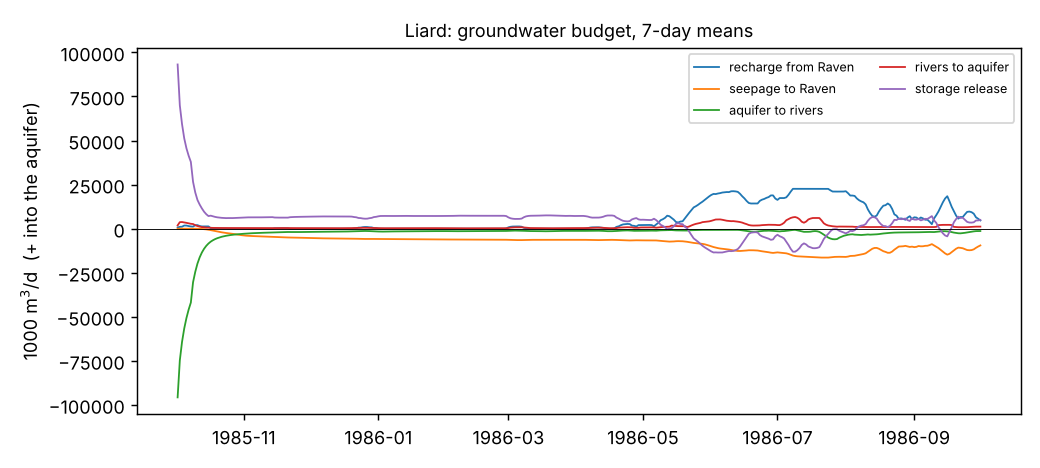
\includegraphics[width=0.9\linewidth]{figures/t1_gw_budget.png}
\caption{\cmd{gw\_budget.png}: the daily groundwater budget of the Liard example (7-day means; positive means into the
aquifer). The large flows of the first weeks are the aquifer adjusting from its initial heads (set by
\cmd{INITIAL\_HEAD\_DEPTH} in \cmd{Liard.rvp}). Afterwards, seepage and discharge to the rivers return the recharge, and
storage takes up the difference.}\label{fig:t1budget}\end{figure}
\begin{figure}[!htbp]\centering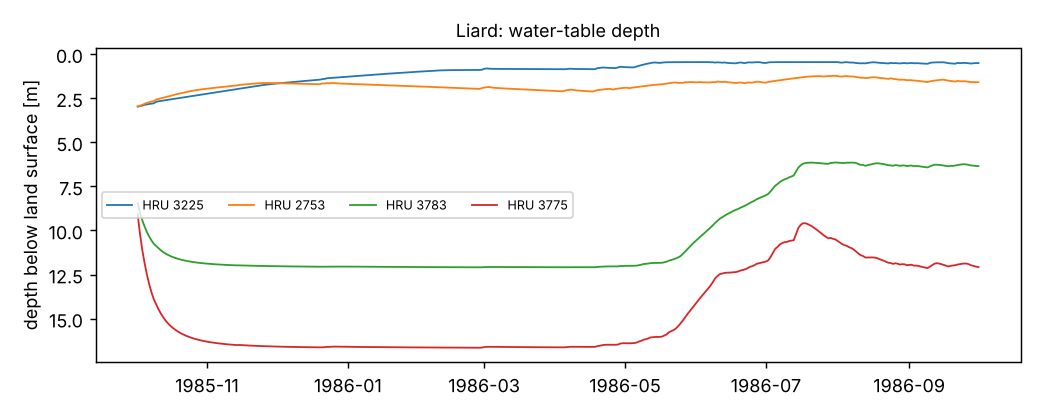
\includegraphics[width=0.9\linewidth]{figures/t1_gw_watertable.png}
\caption{\cmd{gw\_watertable.png}: water-table depth under the two shallowest and the two deepest HRUs. The option
\cmd{--hrus ID ...} of \cmd{plot\_gw.py} chooses other HRUs.}\label{fig:t1wt}\end{figure}
\begin{figure}[!htbp]\centering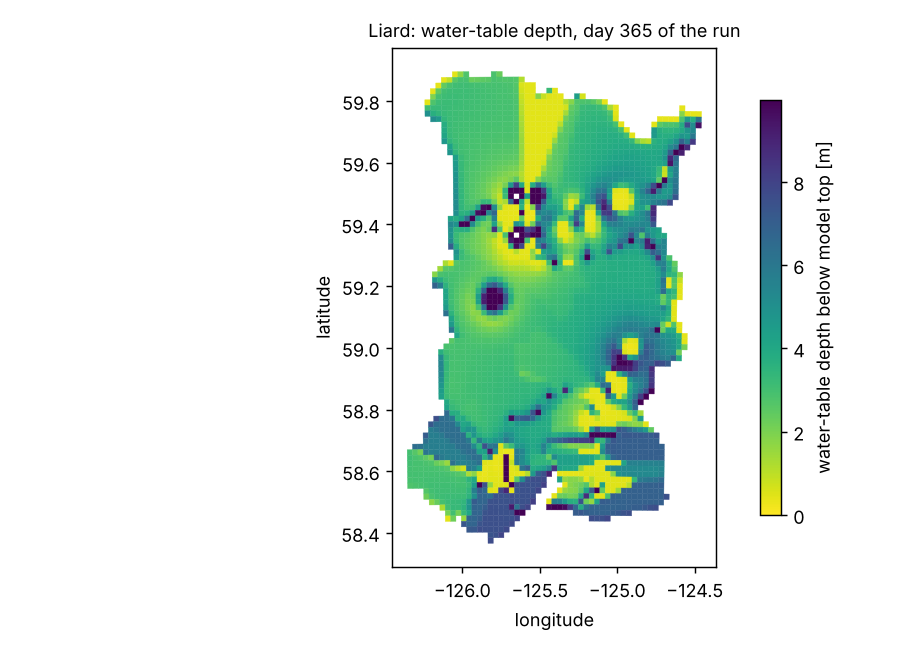
\includegraphics[width=0.72\linewidth]{figures/t1_gw_map.png}
\caption{\cmd{gw\_map.png}: water-table depth in every active column, at the last head field saved in
\cmd{out/mf6/gwf.hds}, on the cells of \cmd{out/mf6/grid\_cells.geojson}. The command \cmd{:HeadSaveFrequency} in
\cmd{Liard.rvg} sets how often MODFLOW saves the heads.}\label{fig:t1map}\end{figure}
\begin{trouble}
\cmd{ModuleNotFoundError: No module named \textquotesingle{}pandas\textquotesingle} (or numpy, matplotlib): the virtual environment is not active in this
terminal. Type \cmd{source \textasciitilde/raven-venv/bin/activate} (Step~\ref{st:python}).
\end{trouble}
\begin{note}[Reading MODFLOW's files yourself]
\cmd{out/mf6/gwf.hds} is a standard MODFLOW~6 head file and \cmd{gwf.dis.grb} its grid file. With FloPy,
\cmd{flopy.utils.HeadFile(\textquotesingle out/mf6/gwf.hds\textquotesingle).get\_data()} returns the last head field. \cmd{grid\_cells.geojson} holds
all cells in longitude and latitude, with their number and an \cmd{active} flag. It opens in any GIS program.
\end{note}

% 06_full_run.tex - the optional 20-year run, and where to go next
\section{The full run (optional)}

\step{Run the full \V{t1:fullYears} years}\label{st:full}
Make a second copy of the example. It keeps the full duration of \V{t1:fullDays} days:
\begin{shell}
$ cp -r $WS/model/start $WS/work_full
$ cd $WS/work_full
$ $RAVEN Liard -o out/
\end{shell}
\see the same progress lines as in the one-year run. The run takes about \V{t1:fullmin}~minutes on the computer that made
this workshop. At the end it prints \msg{Exiting Gracefully: Successful Simulation}.

\step{Check the full run}
\term{t1_audit_full.txt}
\begin{tocheck}
Over \V{t1:fullYears} years: \V{t1:fullUnconv} unconverged steps and a cumulative MODFLOW residual of \V{t1:fullRes} of
the gross flow. The streamflow at the gauges 10BE004, 10BE005 and 10BE010 has Nash--Sutcliffe efficiencies of
\V{t1:fullNSE10BE004}, \V{t1:fullNSE10BE005} and \V{t1:fullNSE10BE010} (in \cmd{out/Diagnostics.csv}; 1 is a perfect fit).
\end{tocheck}

\section{Where to go next}
Workshop~2 builds a groundwater model for a Raven model of your own, from the start. The file \cmd{README.md} in
\cmd{model/start} describes how the Liard example was set up.

\end{document}
